\documentclass[11pt]{article}

\usepackage{../algebra}

\begin{document}

\coverpage{6}

% hw problem 1 -----------------------------------------------------------------

\newpage
\section*{Homomorphisms between clocks}
    \problem{
        Find all homomorphisms from $\Z _{12}$ to $\Z _{15}$.
    }
    \proof{
        I spent a fair bit of time on the next problem so I didn't get a chance to fully explore this one.
        I have found two homomorphisms but was unable to prove that they are the only two.
        I look forward to reading the solutions.
        Here are my two maps.
        There is, of course, the trivial map sending everything in $\Z _{12}$ to $0 \in Z_{15}$.
        The only interesting one I found can be expressed as $f(k) = 5 * (k \mod 3)$ 5 times the remainder of $k$ divided by 3.
        Writing it out directly, elements of the set $\{ 0, 3, 6, 9 \}$ are taken to $0 \in \Z _{15}$,
        $\{ 1, 4, 7, 10 \}$ are taken to $5 \in \Z _{15}$, and $\{ 2, 5, 8, 11 \}$ are taken to $10 \in \Z_{15}$.
    }

% hw problem 2 -----------------------------------------------------------------

\begin{exercise}{74}{13}
    \problem{
        If $G$ is a finite abelian group (note I dropped the $n$ here so I could use that variable in my proof) and $\varphi : G \to G$ is defined by $\varphi (a) = a^m$ for all $a \in G$, find the necessary and sufficient condition that $\varphi$ be an isomorphism of $G$ onto itself.
    }
    \proof{
        This was a fun problem, here is what I came up with!
        Before establishing the conditions, let's discuss some stuff.
        Note that for any $m$, the map $\varphi$ must be homomorphism.
        Consider any $a,b \in G$, then $\varphi (ab) = (ab)^m = a^m b^m = \varphi (a) \varphi (b)$ where the crucial equality $(ab)^m = a^m b^m$ is made possible since $G$ is abelian. 
        Also we will only consider $0 \leq m < |G|$ since any $m$ outside that range has a brother in the range that performs the same operation (since any element to the power of $|G|$ is the identity). \parspace
        I claim that any finite group $G$ can be decomposed into cyclic subgroups $H_1, H_2, ..., H_k$ such that their union is $G$ and the only common member between any two subgroups is $e \in G$. \parspace
        I will not give a rigorous proof of this claim but I do provide the following informal reasoning.
        For $h_j \in G$, define the cyclic subgroup $H_j = (h_j)$.
        Consider the set of all cyclic subgroups $\mathbb{H} = \{ H_j = (h_j) \mid h_j \in G \}$.
        Then ignore any subgroup $H_i$ that is a subgroup of another subgroup $H_j$.
        Let this collection of subgroups be $H_1, H_2, ..., H_k$.
        Certainly their union is the entire group since we only forgot subgroups that were included in other subgroups.
        And we can deduce that their only common element is the identity because if there were a common element, it's powers would be in both subgroups and one would be a subgroup of the other.
        The example that I thought about while writing this was $\Z_{12}$.
        Here, the subgroup $(4) \leq (2)$. \parspace
        Now we present the conditions.
        Consider a finite, abelian group $G$ of order $n$, $G'$s decomposition into the ``mostly'' disjoint subgroups $H_1, H_2, ... , H_k$, and the function $\varphi : G \to G$ defined by $\varphi (a) = a^m$.
        The map $\varphi$ is an isomorphism if and only if we have $(m, |H_j|) = 1$ for all $H_j \in \{ H_1, H_2, ..., H_k \}$.
        We will do this in two stages. 
        First we will consider the cyclic group $\Z_n$ and then we will show that any cyclic group of order $n$ is isomorphic to $\Z_n$. \parspace
        For the cyclic group $\Z _n$ generated by $(1)$, the function $\varphi$ is realized as $\varphi (k) = [mk]$.
        We show that $\varphi$ is an isomorphism if and only if $(m, n) = 1$.
        We will start by supposing that $(m, n) = 1$.
        We already know $\varphi$ is a homomorphism and since $\varphi$ is a map from a finite set to itself we only need to show that $\varphi$ is 1-1 to prove that $\varphi$ is a bijection, and hence an isomorphism.
        Pick any $a, b \in \Z_n$ such that $\varphi (a) = \varphi (b)$ then $[ka] = [kb]$.
        Splitting the product, gives $[k] [a] = [k] [b]$ and cancelation gives $[a] = [b]$ so $\varphi$ is 1-1 so we conclude $\varphi$ is an isomorphism. \parspace 
        Going the other direction, we will show the contrapositive.
        That is, suppose $(m, n) \neq 1$ and we will show that $\varphi$ is not an isomorphism.
        In particular, we will show $\varphi$ is not 1-1.
        Since $(m, n) \neq 1$, there exists some $x > 1$ such that $x \mid m$ and $x \mid n$ (then $n/x$ is an integer and there exists a $d \in \Z$ such that $xd = m$).
        Then evaluate $\varphi (n/x) = [m n/x] = [xd n/x] = [dn] = [0]$ which is congruent to 0 mod $n$.
        But $\varphi (0) = [0]$ so we have distinct inputs that map to the same output so $\varphi$ cannot be 1-1.
        So we have shown that $\varphi$ is an isomorphism if and only if $(m, n) = 1$. \parspace 
        Now we show that any cyclic group of order $n$ is isomorphic to $\Z _n$.
        Consider a cyclic group of order $n$: $F = \{ e, f, f^2, ..., f^{n-1} \}$.
        The function $\psi : F \to \Z _n$ defined by $\psi (f^i) = [i]$ is an isomorphism.
        First we show $\psi$ is a homomorphism: $\psi (f^i f^j) = \psi (f^{i+j}) = [i+j] = [i] + [j] = \psi (f^i) + \psi (f^j)$.
        Then we show that $\psi$ is 1-1 (equal and finite cardinality means we can ignore onto when establishing bijectivity).
        Pick $\psi (f^i) = \psi (f^j) \implies [i] = [j]$ which means $f^i = f^j$.
        So $F \cong \Z_n$, which means that we can use the map $\psi ^{-1} \circ \varphi \circ \psi : F \to F$ as a self-isomorphism if $\varphi$ is a self-isomorphism. 
        But we just showed exactly when $\varphi : \Z_n \to \Z _n$ is a self-isomorphism. \parspace 
        Now we return to the problem at hand: showing that $\varphi : G \to G$ is an isomorphism if and only if $(m, |H_j|) = 1$ for all $H_j \in \{ H_1, H_2, ..., H_k \}$.
        Because of all the work we have put in, this turns out to be quite easy and we will use a similar structure to the proof for $\Z _n$.
        Going to the left, we use the contrapostive: suppose there exists an $H_i \in \{ H_1, H_2, ..., H_k \}$ such that $(m, |H_i|) > 1$.
        Then $\varphi$ is not an isomorphism for elements of $H_i$.
        But $H_i \leq G$ so $\varphi$ can also not be an isomorphism for $G$ (recall if $h$ is not the identity then no other subgroup we care about contains $h$). \parspace 
        Then going to the right, we know that we can define an isomorphism for each $\{ H_1, H_2, ..., H_k \}$ (since they are cyclic) and since they pairwise disjoint (excluding the identity) the map that just operates on $g \in G$ according to the subgroup $H_i$ containing $g$ will also be an isomorphism.
        The operation on the identity is well defined since every homomorphism takes the identity to the identity. 
        So we have shown exactly when $\varphi$ is an isomorphism. \parspace 
        This problem was really fun to explore, I gave it my best shot at providing a rigorous answer and I look forward to reading the solutions!
    }
\end{exercise}


% hw problem 3 -----------------------------------------------------------------

\begin{exercise}{75}{26}
    \problem{
        If $G$ is a group and $a \in G$, define $\sigma _a (g) = a g a^{-1}$.
        We saw in Example 9 of this section that $\sigma _a$ is an isomorphism of $G$ onto itself, so $\sigma _a \in A(G)$, the group of all $1-1$ mappings of $G$ (as a set) onto itself.
        Define $\psi: G \to A(G)$ by $\psi (a) = \sigma _a$ for all $a \in G$.
        Prove that \\
        \indent {\bf (a)} $\psi$ is a homomorphism of $G$ into $A(G)$. \\
        \indent {\bf (b)} $\ker \psi = Z(G)$ the center of $G$.
    }
    \proof{
        \parspace {\bf (a)} We wish to show that $\psi$ is a homomorphism.
        That is, we must show that $\psi (ab) = \psi (a) \psi (b)$ for all $a,b \in G$.
        On the LHS, we have $\psi (ab) = \sigma _{ab}$ and on the RHS we have $\psi (a) \psi (b) = \sigma _a \circ \sigma _b$.
        For the LHS to equal the RHS we must have $\sigma _{ab} (g) = (\sigma _a \circ \sigma _b) (g)$ for all $g \in G$.
        Fix any $g \in G$, then $\sigma _{ab} (g) = (ab) g (ab)^{-1} = ab g b^{-1} a^{-1} = \sigma _a (b g b^{-1}) = \sigma _a (\sigma _b (g)) = (\sigma _a \circ \sigma _b) (g)$.
        Since $g$ was arbitrary in $G$, we have shown the equality between maps $\sigma _{ab} = \sigma _a \circ \sigma _b$ which means $\psi$ is a homomorphism. \parspace
        {\bf (b)} Now we want to show that $\ker \psi = Z(G)$.
        Let's write their definitions.
        We know $\ker \psi := \{ a \in G \mid \psi (a) = id \in A(G) \} \subset G$ and that $Z(G) := \{ a \in G \mid ag = ga \text{ for all } g \in G \}$.
        We will show equality by showing inclusion in both directions.
        Going to the left, pick any $a \in \ker \psi$, then $\psi (a) = id \in A(G)$.
        Also, by definition, $\psi (a) = \sigma _a$ this gives the equality of maps $\sigma _a = id$.
        Then we have $\sigma _a (g) = id(g) = g$ for all $g \in G$.
        By definition, $\sigma _a (g) = a g a^{-1}$ so we also have $a g a^{-1} = g$ for all $g \in G$.
        Right multiplying by $a$ gives $ag = ga$ for all $g$, which is exactly the condition for membership in $Z(G)$.
        Therefore, $a \in Z(G)$ and since $a$ was arbitray in $\ker \psi$ we have the inclusion $\ker \psi \subset Z(G)$. \parspace
        We now show the other inclusion $Z(G) \subset \ker \psi$.
        Fix any $b \in Z(G)$ then $bg = gb$ for every $b \in G$.
        Right multplying by $b^{-1}$ gives the equality $b g b^{-1} = g$ for all $b \in G$.
        The LHS is exactly $\sigma _b (g)$ so we have just shown that $\sigma _b (g) = g$ for every $b$.
        But then $\sigma _b$ performs the same actions as the identity map $id \in A(G)$ so we have $\sigma _b = id$.
        Further, $\sigma _b = \psi (b)$ so we also have $\psi (b) = id \in A(G)$, which is the condition for membership in $\ker \psi$.
        By arbitrariness of $b$, we have shown $Z(G) \subset \ker \psi$.
    }
\end{exercise}

% hw problem 4 -----------------------------------------------------------------

\newpage
\section*{Heisenberg to plane}
    \problem{
        Find an epimorphism the Heisenberg group $\Heisen$ onto $\R ^2$.
    }
    \proof{
        Consider the function $\varphi : \Heisen \to \R ^2$ which maps a matrix
        $A = \begin{bmatrix} 1 & x & z \\ 0 & 1 & y \\ 0 & 0 & 1 \end{bmatrix} \in \Heisen$
        to the point $(x, y) \in \R ^2$.
        For $\varphi$ to be an epimorphism, we must verify that $\varphi$ is both surjective and a homomorphism.
        For $\varphi$ to be surjective, for every point in $\R ^2$ we must have a matrix in $\Heisen$ such that $\varphi$ maps the matrix to the point.
        For the point $(a, b) \in \R ^2$, choose the matrix
        $A = \begin{bmatrix} 1 & a & 0 \\ 0 & 1 & b \\ 0 & 0 & 1 \end{bmatrix}$.
        Then $\varphi (A) = (a, b)$ as desired.
        Now let's verify that $\varphi$ is a homomorphism.
        We must check that $\varphi (A A') = \varphi (A) \varphi (A')$ for all $A, A' \in \Heisen$.
        $$
        A A' =
        \begin{bmatrix}
            1 & x & z \\
            0 & 1 & y \\
            0 & 0 & 1
        \end{bmatrix}
        \begin{bmatrix}
            1 & x' & z' \\
            0 & 1 & y' \\
            0 & 0 & 1
        \end{bmatrix}
        =
        \begin{bmatrix}
            1 & x'+x & z'+y'x+z \\
            0 & 1 & y'+y \\
            0 & 0 & 1
        \end{bmatrix}
        $$
        On the LHS, $\varphi (A A') = (x' + x, y' + x)$.
        Then on the RHS, we have $\varphi (A) \varphi (A') = (x, y) + (x', y') = (x+x', y+y') = (x'+x, y'+y)$.
        So the LHS equals the RHS and $\varphi$ is a homomorphism.
    }

% hw problem 5 -----------------------------------------------------------------

\newpage
\section*{Klein group}
    \problem{
        Show that the group $Sym (R)$ where $R$ is a rectangle that is not a square is isomorphic to the product $\Z _2 \times \Z _2$.
    }
    \proof{
        We know the elements of $\Z _2$ so we know the elements of $\Z _2 \times \Z _2$ and the group opertion it is endowed with.
        We must explore the group $Sym (R)$.
        Certainly $Sym (R) \leq D_8$ (where $S$ is a square) for every symmetry of a rectangle is also a symmetry of a square.
        Figure \ref{fig:sym} depicts the axis of symmetries of a rectangle $R$.
        Together with the identity transformation, there are four.
        Since $Sym (R) \leq D_8$ let's give the four transformations the same names that we call them in $D_8$.
        Namely, $Sym (R) := \{ e, r^2, f, fr^2 \}$.

        \begin{figure}[h]
            \centering
            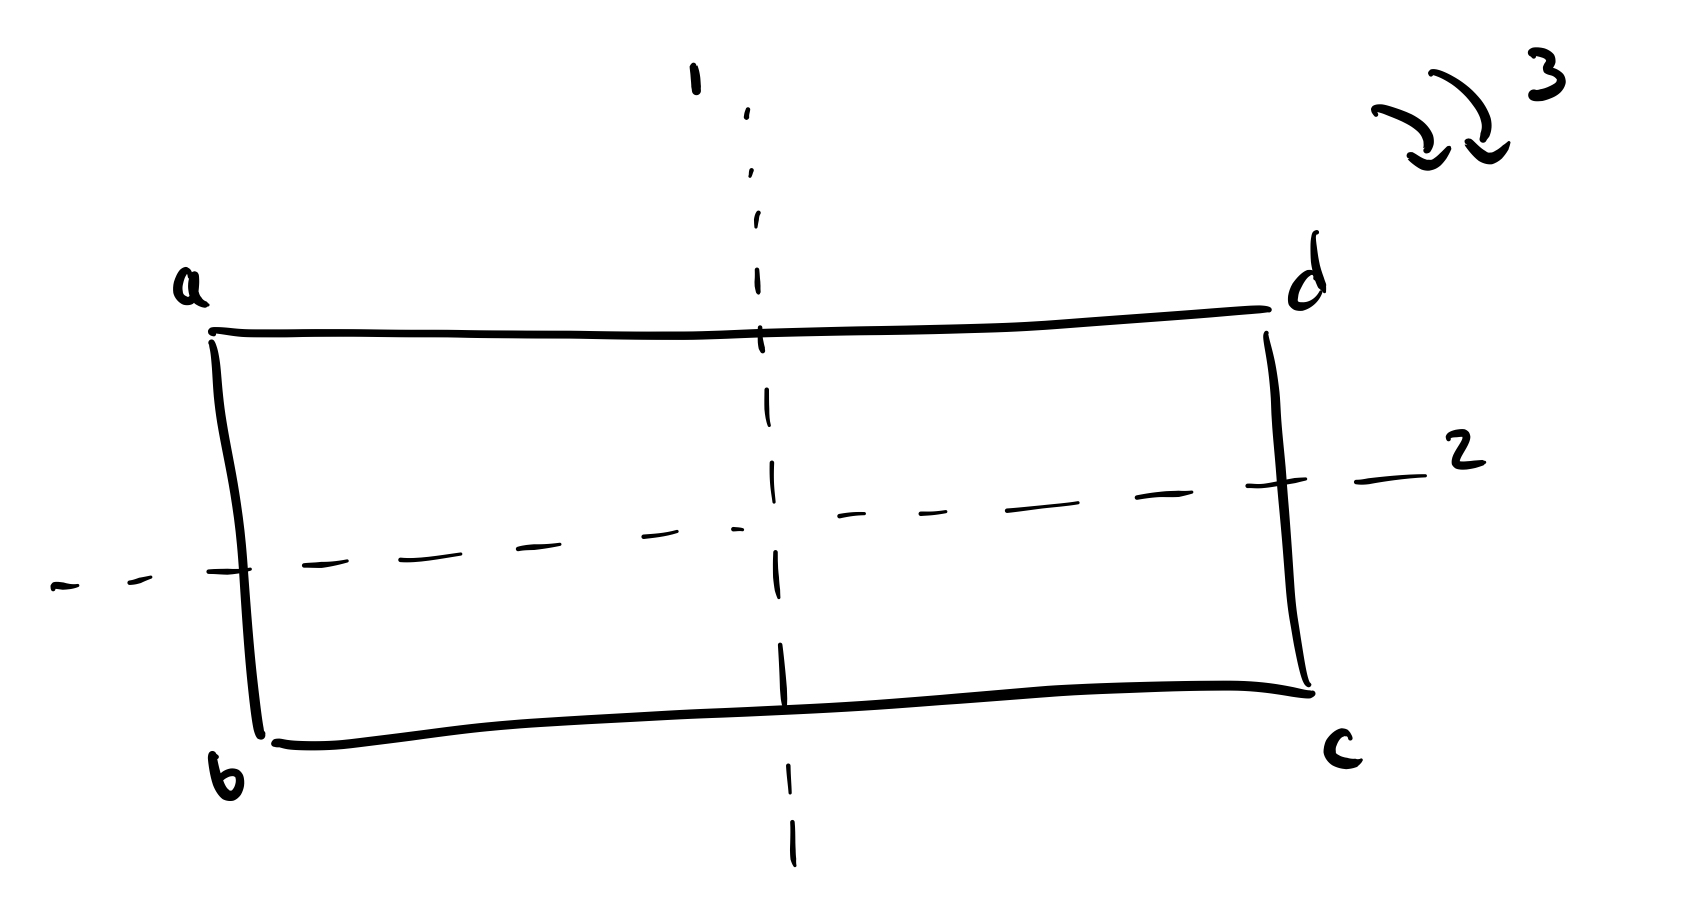
\includegraphics[width=0.5\textwidth]{img/sym}
            \caption{Symmetries of a rectangle $R$}
            \label{fig:sym}
        \end{figure}

        Figure \ref{fig:iso} defines a map $\varphi: Sym (R) \to \Z _2 \times \Z _2$.
        Just from the figure, we know that $\varphi$ is a bijection.

        \begin{figure}[h]
            \centering
            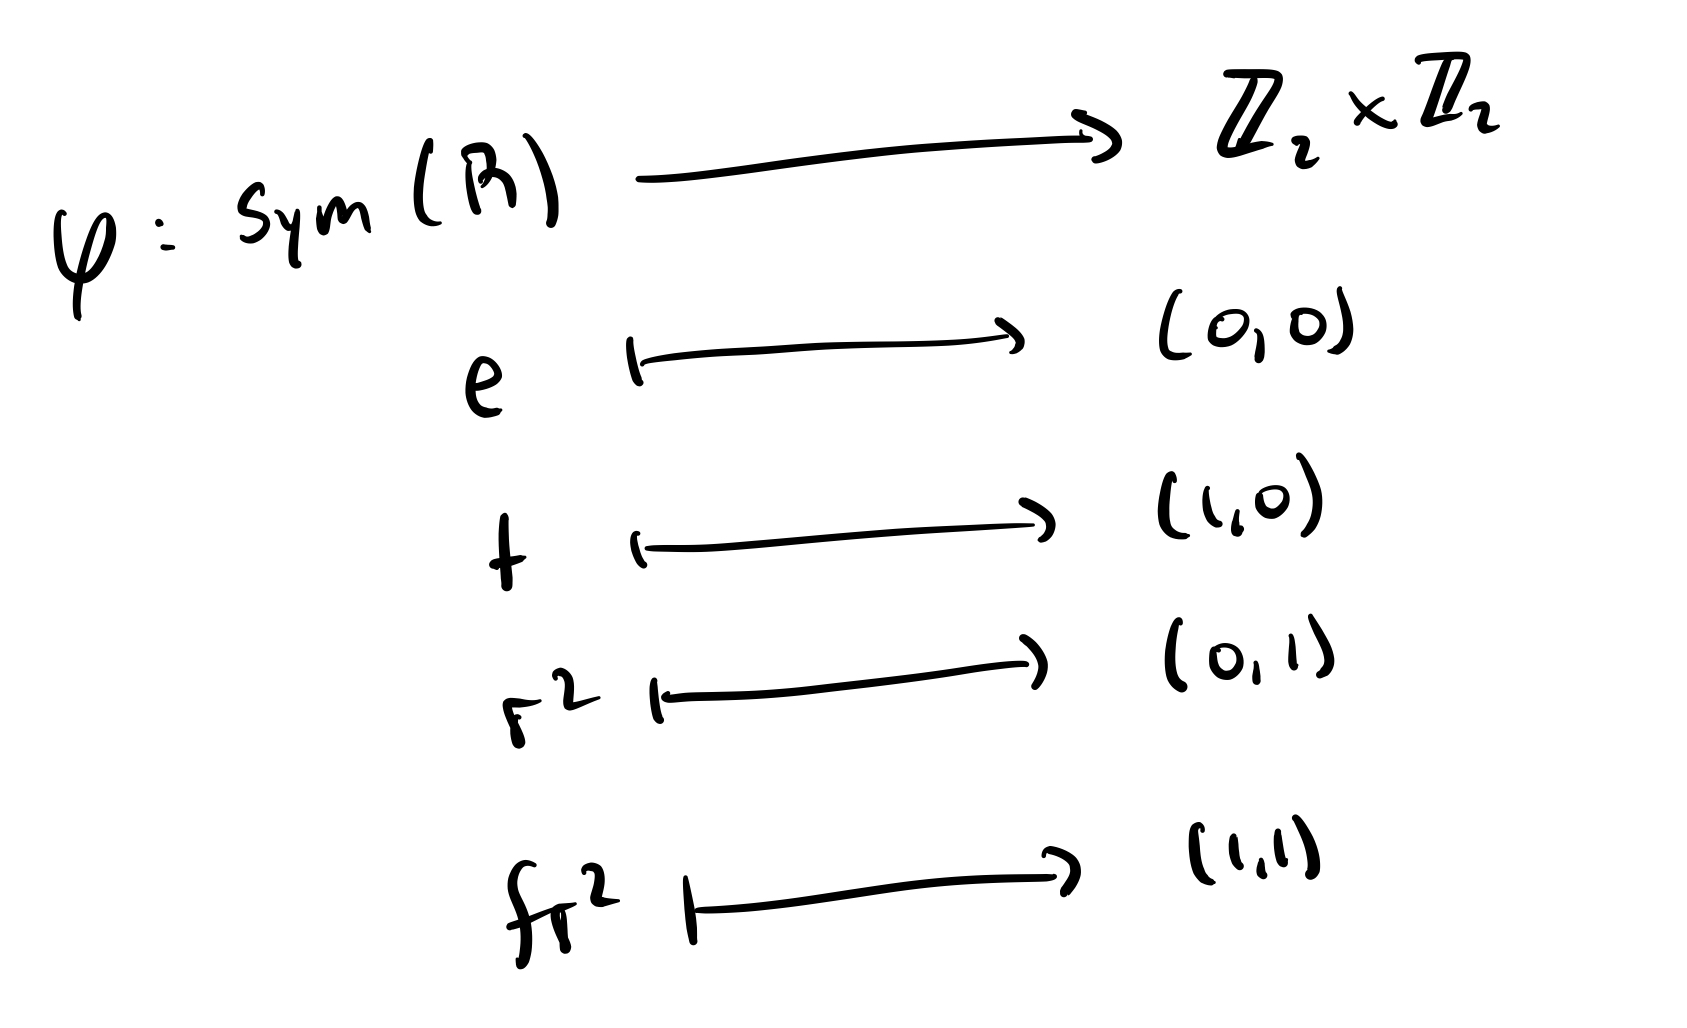
\includegraphics[width=0.4\textwidth]{img/iso}
            \caption{Isomorphism between $Sym (R)$ and $\Z _2 \times \Z _2$}
            \label{fig:iso}
        \end{figure}

        To verify that $\varphi$ is an isomorphism, we must verify that $\varphi$ is a homomorphism.
        Before doing this, note that $\Z _2 \times \Z _2$ and $Sym (R)$ are abelian.
        We can check $Sym (R)$ by verifying that $ f r^2 = r^2 f$.
        Since each group is abelian, we only need to check one ``ordering'' of each pair of elements.
        Now we verify that $\varphi$ respects the group structure.
        \begin{align*}
            \varphi (e) + \varphi (x) &= (0, 0) + \varphi (x) = \varphi (x) = \varphi (e x) \text{ for any } x \in Sym(R) \\
            \varphi (f) + \varphi (r^2) &= (1,0) + (0,1) = (1,1) = \varphi (f r^2) \\
            \varphi (f) + \varphi (fr^2) &= (1,0) + (1,1) = (0,1) = \varphi (r^2) = \varphi (ff r^2) \\
            \varphi (f r^2) + \varphi (r^2) &= (1,1) + (0,1) = (1,0) = \varphi (f) = \varphi (f r^4) \\
        \end{align*}
    }

\end{document}
